% !TEX root = ../YourName-Dissertation.tex

\chapter{Direct Measurement of the Neutrino Mass with Cyclotron Radiation Emission Spectroscopy}

\section{Introduction}

\section{Cyclotron Radiation Emission Spectroscopy}

Of the standard physical quantities the one that can be measured with the highest precision is time and the inversely related quantity frequency. In fact it is often advantageous to convert measurements of other physical quantities like mass or length into frequency measurements due to the digital nature of frequency measurements that make them immune to many sources of noise. Atomic clocks, which operate by measuring the frequencies of various atomic transitions, have been used to measure time with astounding relative uncertainties of $10^{-18}$~seconds. The extreme precision possible with frequency measurements is often summarized using the a quote from the Physicist Arthur Schawlow who said advise his students to "Never measure anything but frequency!". 

Neutrino mass measurements using tritium beta-decay are effectively attempting to measure  

\begin{figure}[htbp]
    \centering
    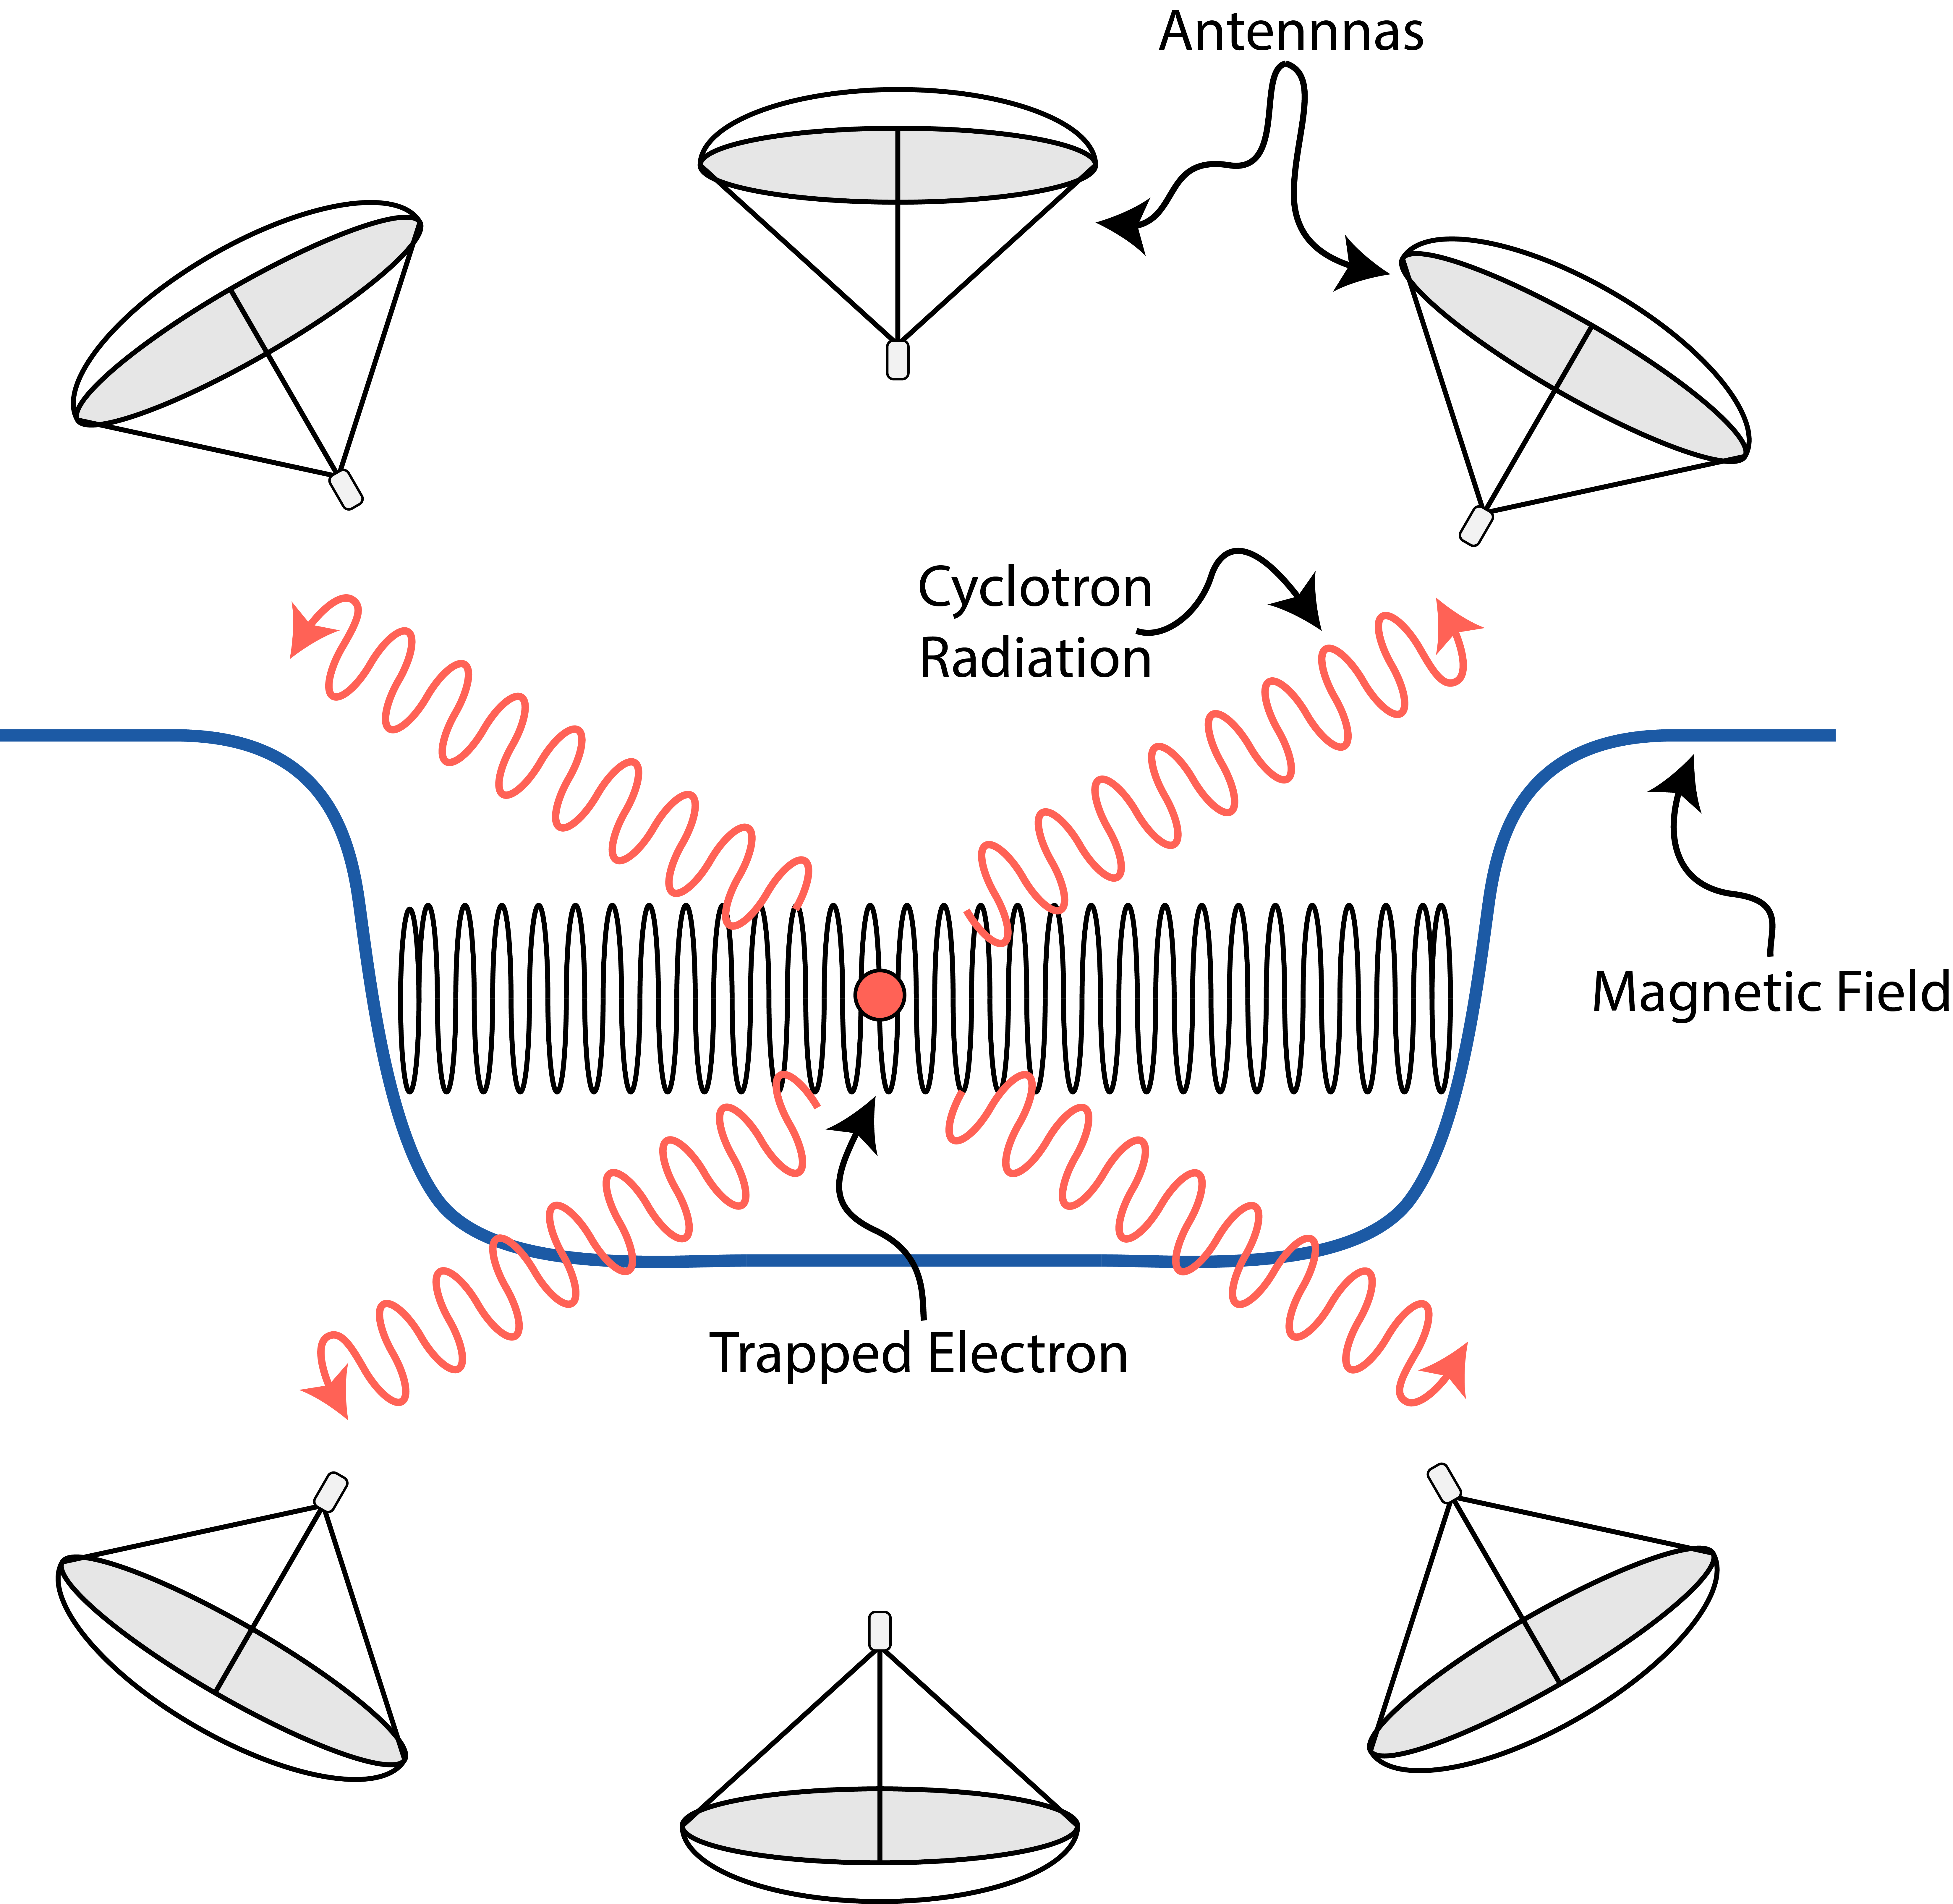
\includegraphics[width=0.5\textwidth]{figs/Chapter-3/230303_cres_cartoon.png}
    \caption{Caption}
    \label{fig:cres_cartoon}
\end{figure}

\subsection{Charged Particles in a Magnetic Trap}

\begin{figure}[htbp]
    \centering
    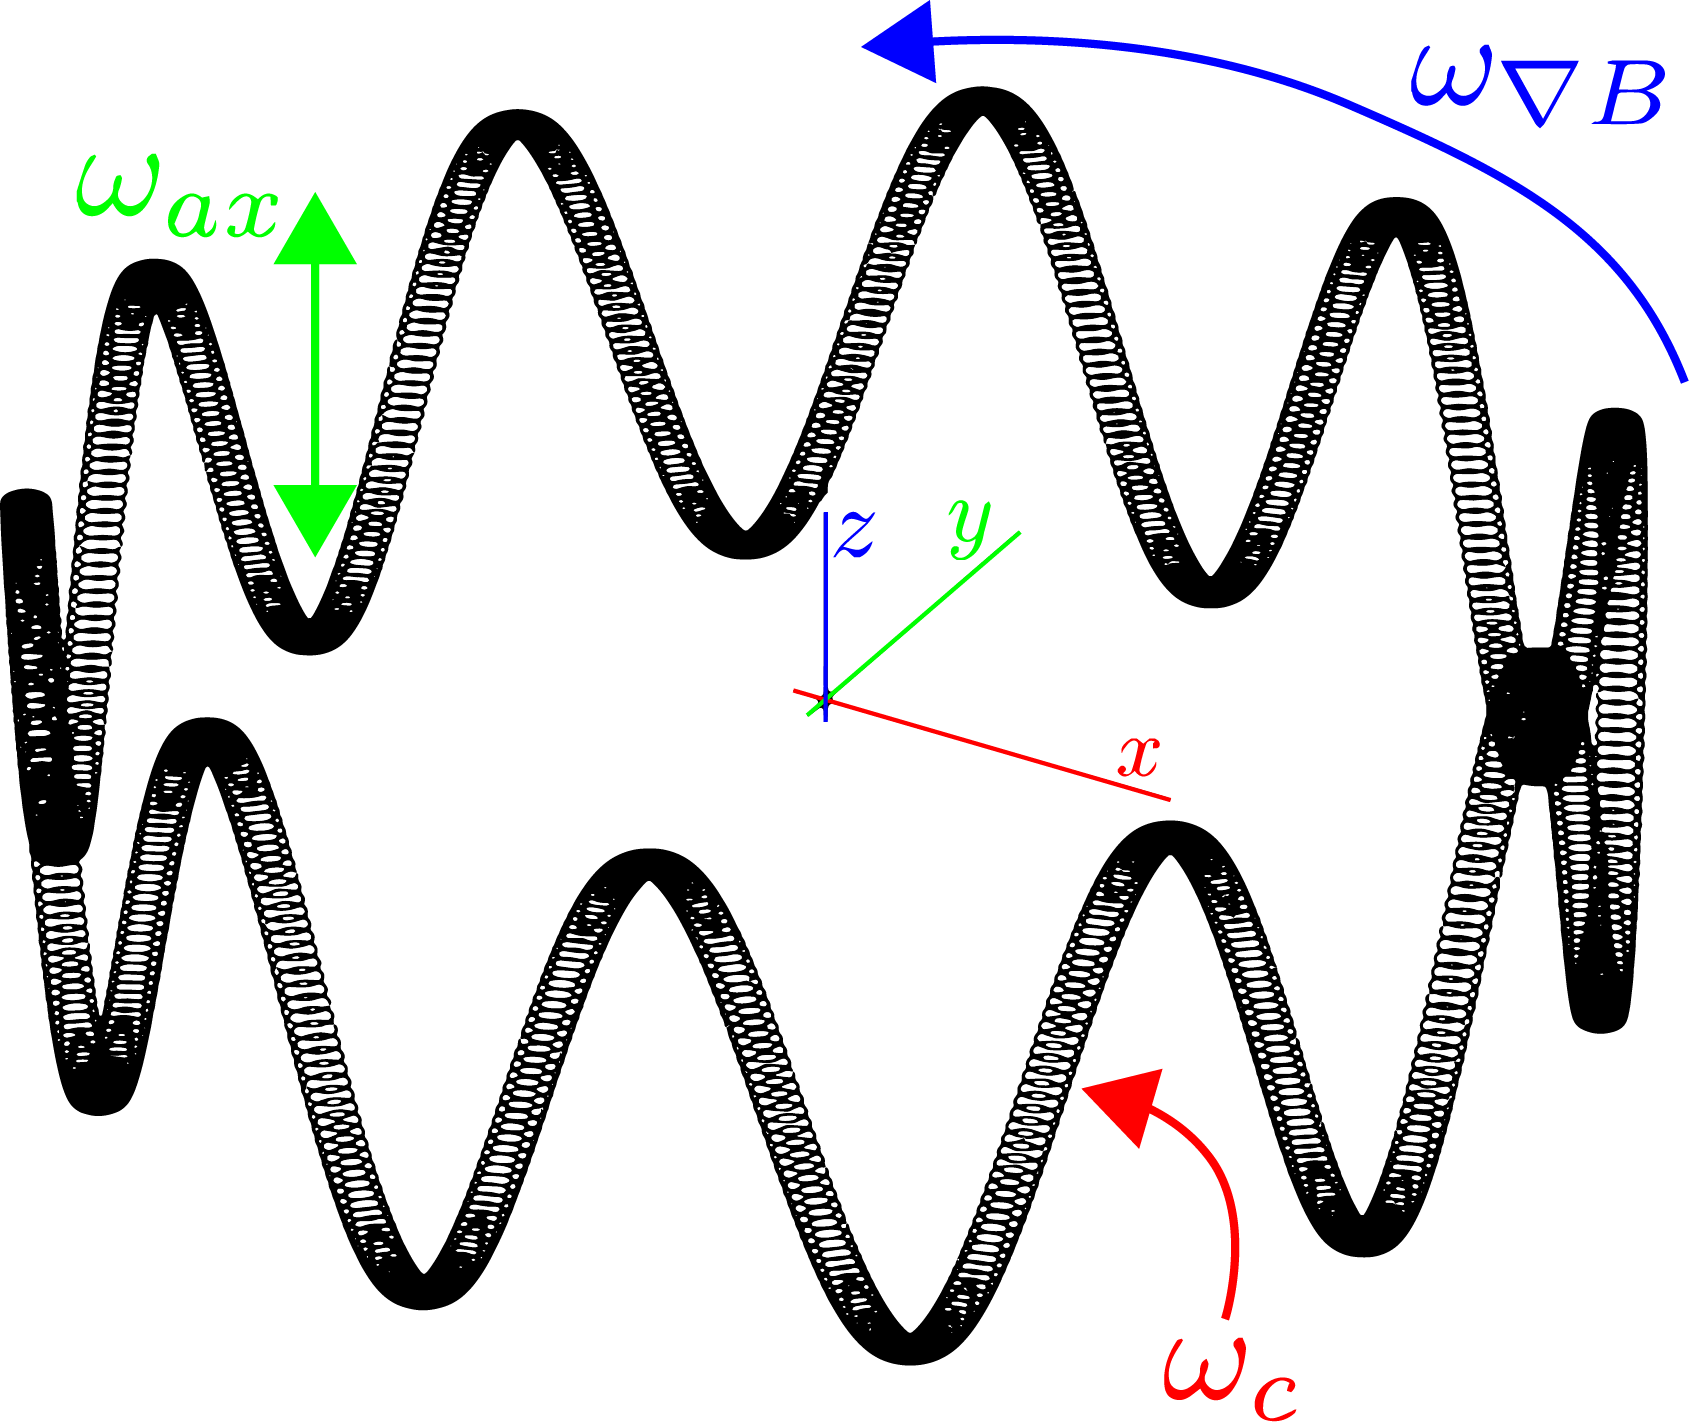
\includegraphics[width=0.5\textwidth]{figs/Chapter-3/230511_trapped_motion.png}
    \caption{Caption}
    \label{fig:chap3-trapped-electron-motion}
\end{figure}

\subsection{Radiation from a Charged Particle}

\section{The Project 8 Collaboration}

\begin{figure}[htbp]
    \centering
    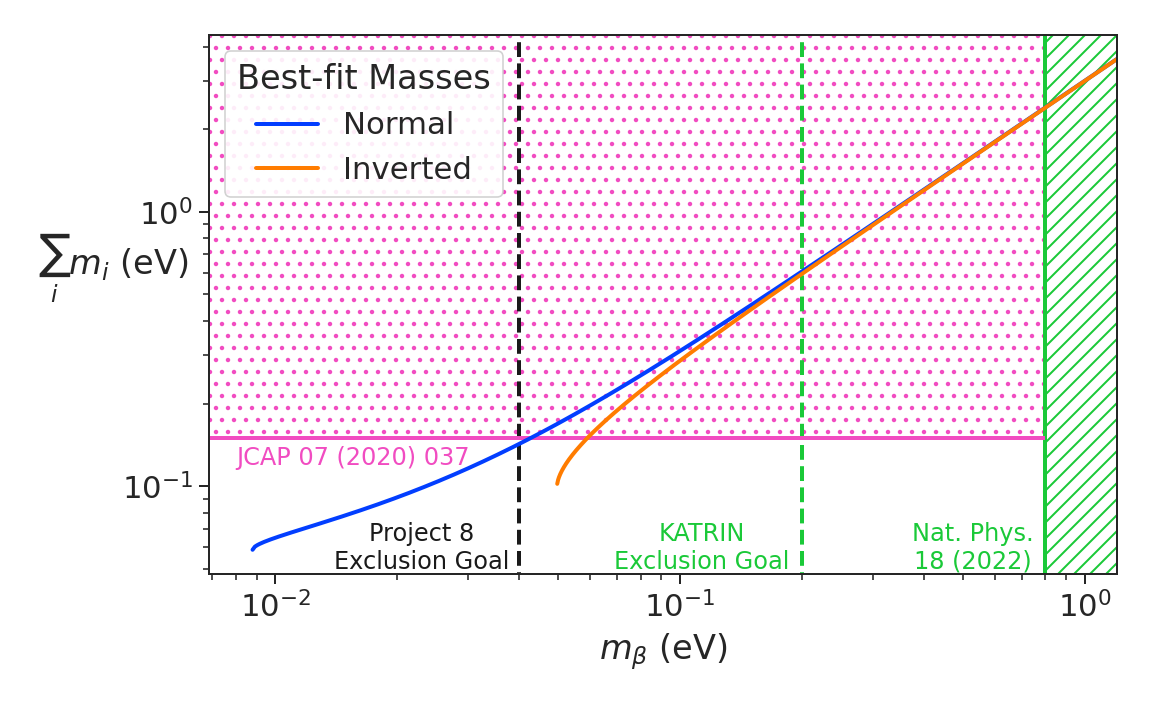
\includegraphics[width=0.7\textwidth]{figs/Chapter-3/230303_sum_nu_mass_vs_m_beta_with_exclusion_and_goal.png}
    \caption{Caption}
    \label{fig:p8_nu_mass_goal}
\end{figure}

\section{First Tritium Beta Decay Spectrum and Neutrino Mass Measurment with CRES}

\subsection{The Project 8 CRES Demonstrator}

\begin{figure}[htbp]
    \centering
    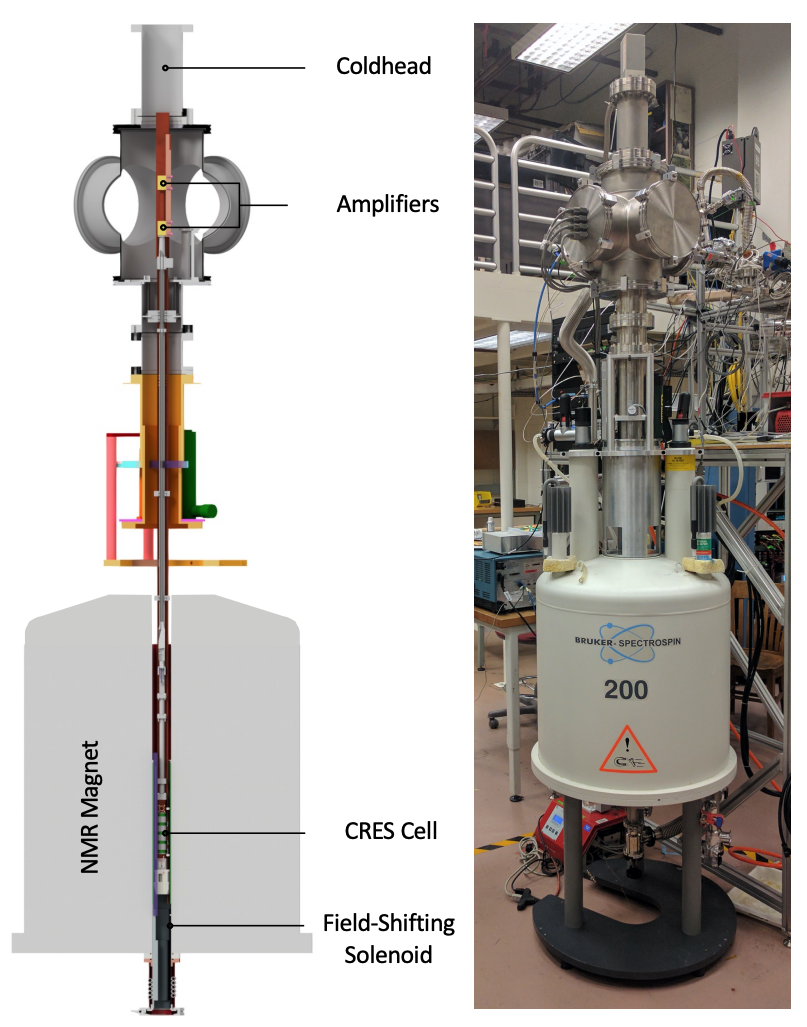
\includegraphics[width=0.7\textwidth]{figs/Chapter-3/phaseII_system.png}
    \caption{Caption}
    \label{fig:phase2_apparatus}
\end{figure}

\begin{figure}[htbp]
    \centering
    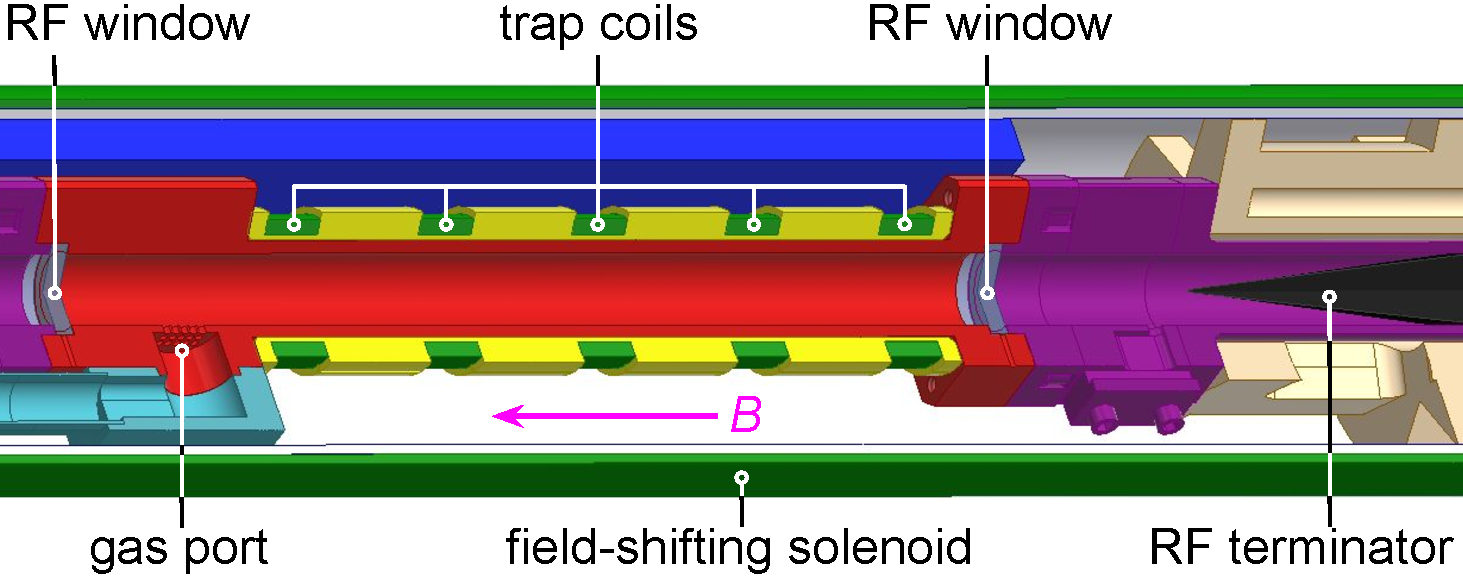
\includegraphics[width=0.8\textwidth]{figs/Chapter-3/apparatus.pdf}
    \caption{Caption}
    \label{fig:phase2_cres_cell}
\end{figure}

\subsection{CRES Track and Event Reconstruction}

\begin{figure}[htbp]
    \centering
    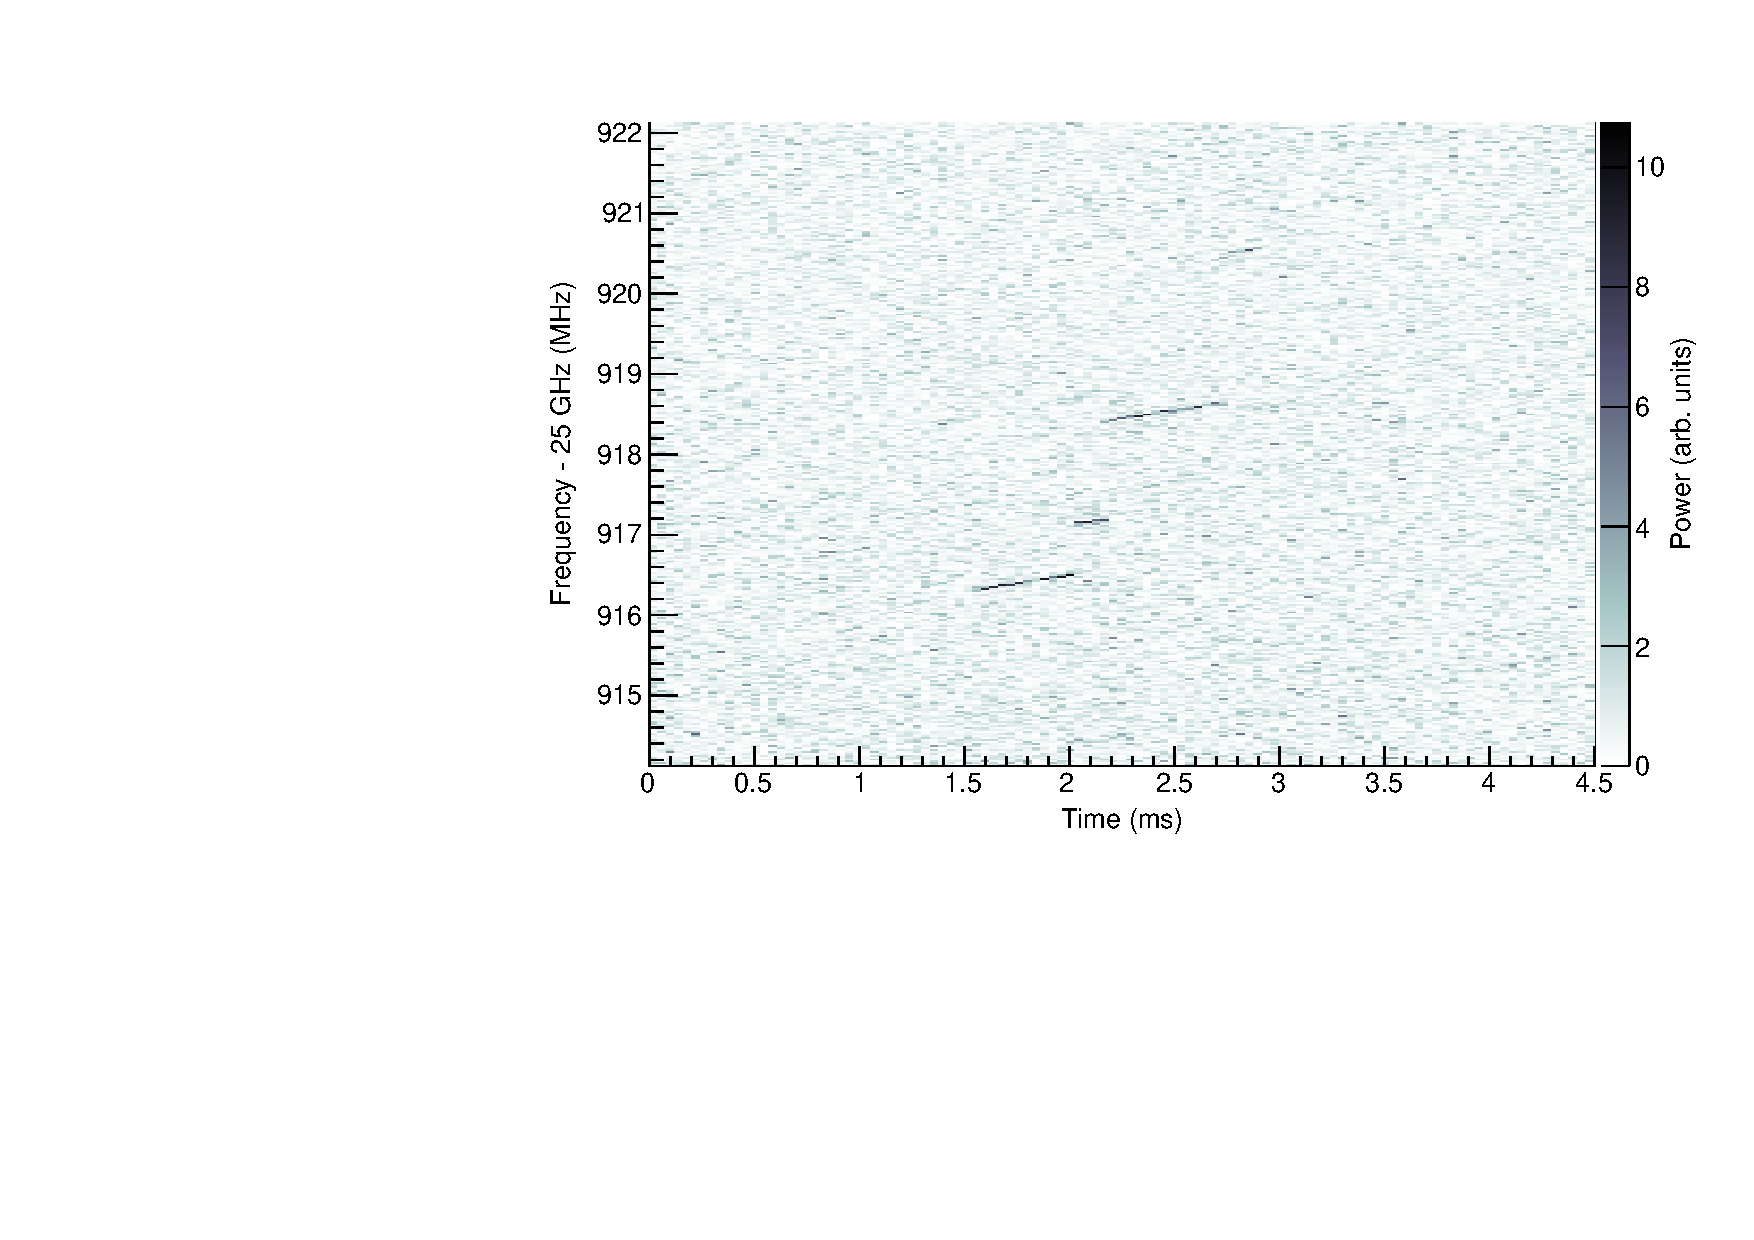
\includegraphics[width=0.7\textwidth]{figs/Chapter-3/T2_Event0.pdf}
    \caption{Caption}
    \label{fig:tritium_event0}
\end{figure}

\subsection{Measurements with Krypton}

\begin{figure}[htbp]
    \centering
    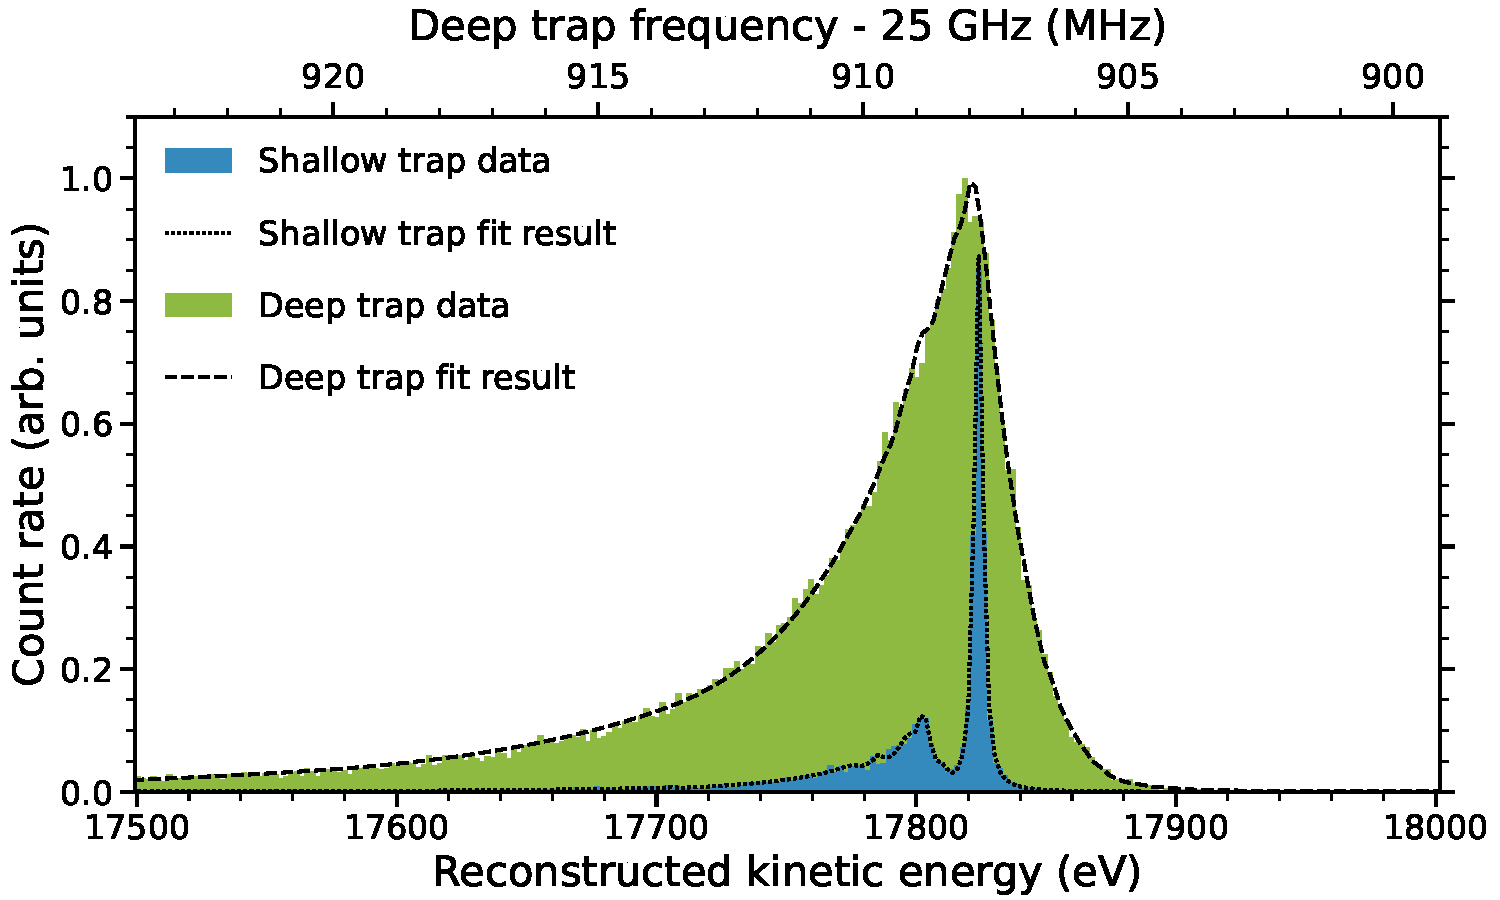
\includegraphics[width=0.7\textwidth]{figs/Chapter-3/kr_fit.pdf}
    \caption{Caption}
    \label{fig:krypton_fit}
\end{figure}

\begin{figure}[htbp]
    \centering
    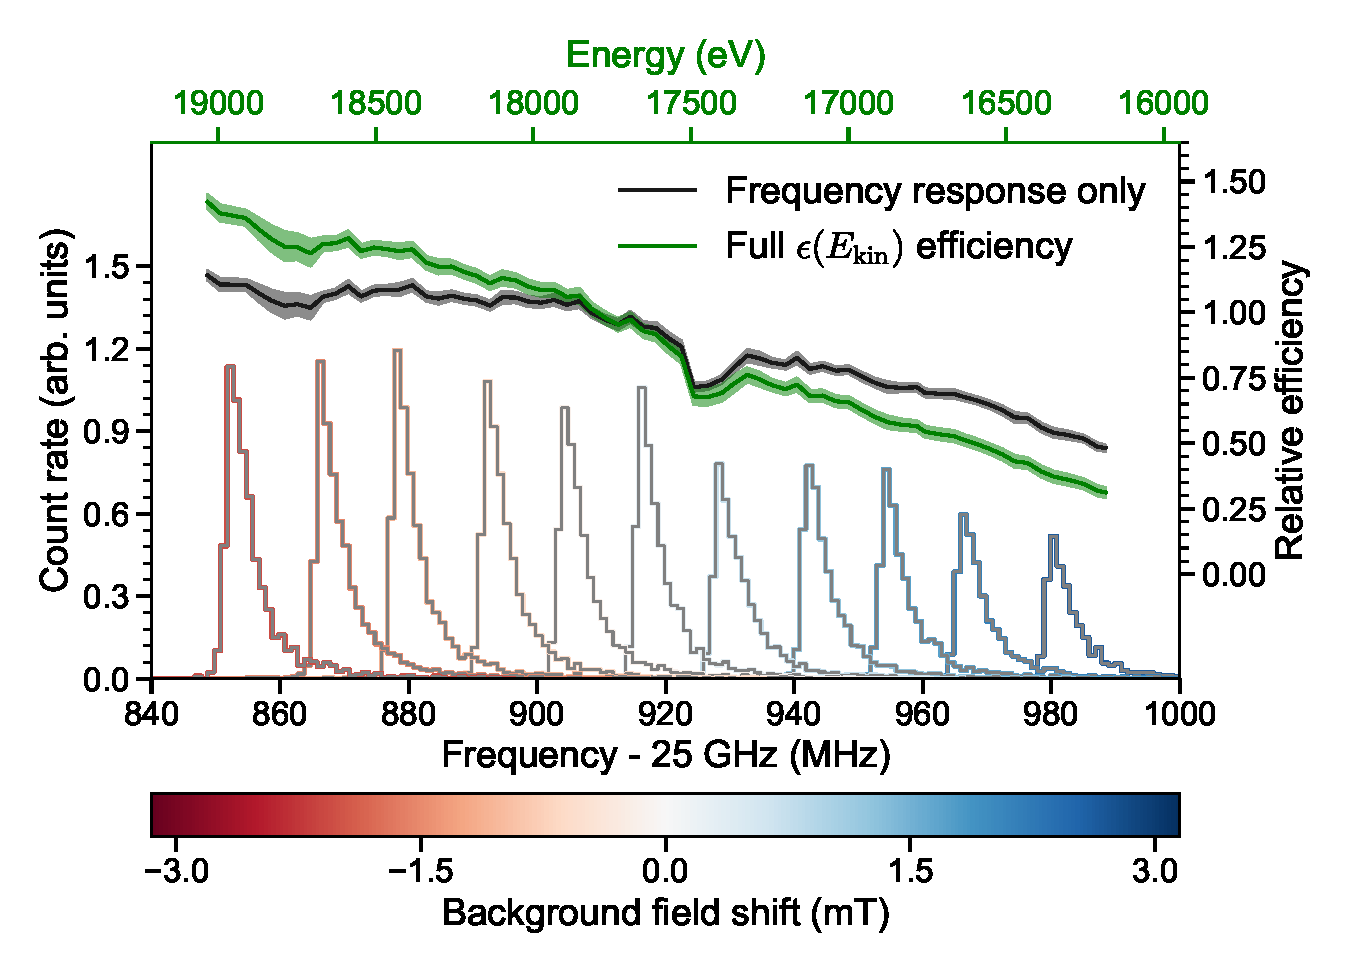
\includegraphics[width=0.7\textwidth]{figs/Chapter-3/fss_for_prl_plot.pdf}
    \caption{Caption}
    \label{fig:fss_plot}
\end{figure}

\subsection{Tritium Spectrum and Neutrino Mass Results}

\begin{figure}
    \centering
    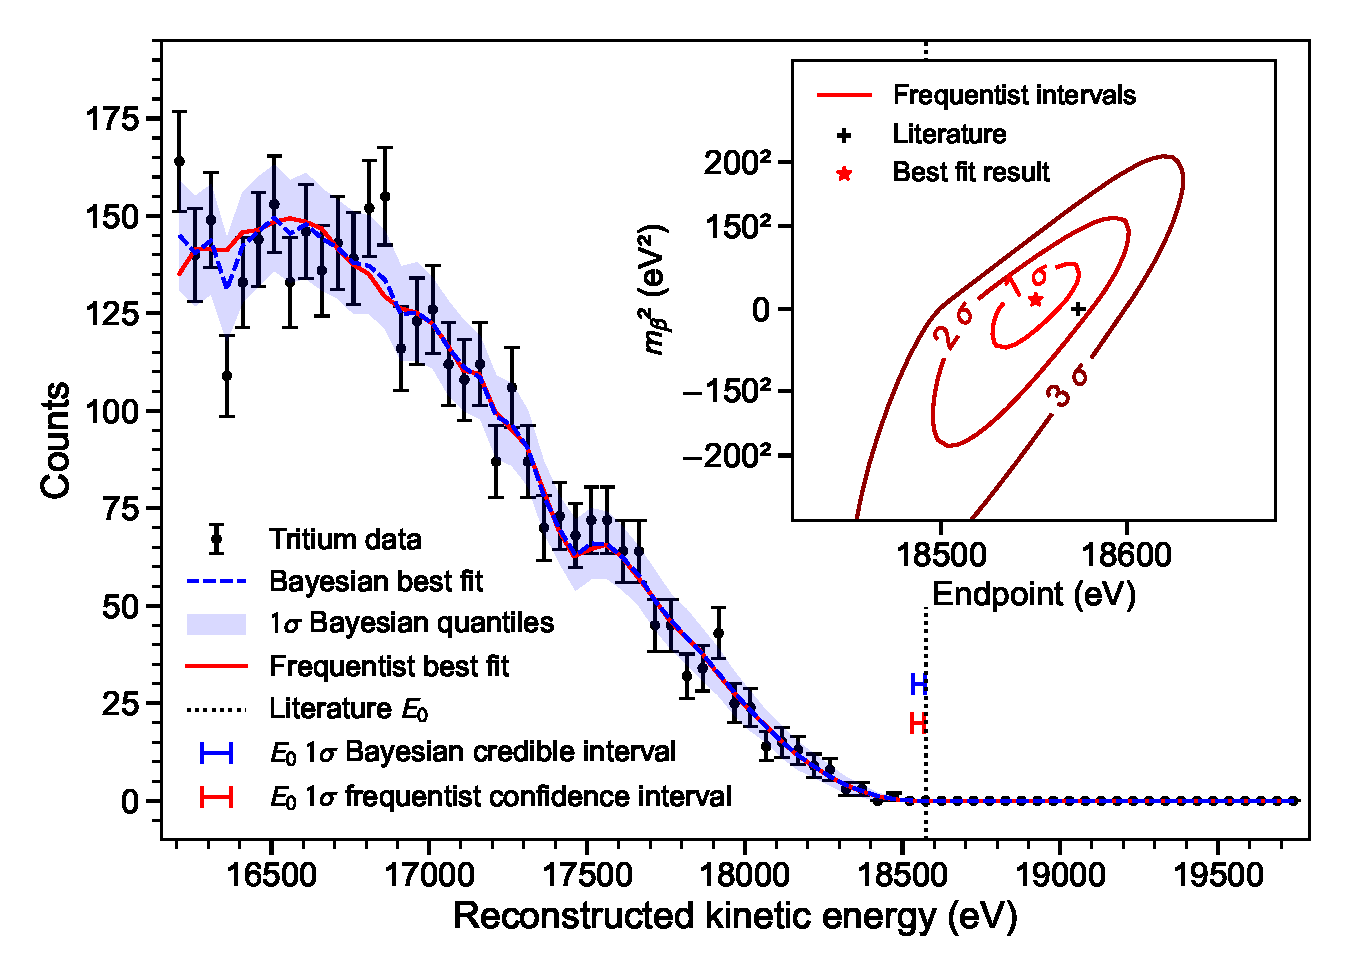
\includegraphics[width=0.7\textwidth]{figs/Chapter-3/12-03-22A_final_E0_real_data_phase_II_tritium_fit_1d.pdf}
    \caption{Caption}
    \label{fig:final_tritium_fit}
\end{figure}

\section{Scalable Approaches to CRES Measurements}
\subsection{The Antenna Array Approach}
\subsection{The Cavity Approach}



